\documentclass[slidestop,compress]{beamer}
\usetheme{Singapore}

\sloppy
%\usepackage[scaled]{helvet}
%\usepackage{eulervm}

\usepackage{fp-eval}
\usepackage{hyperref}
\usepackage{fancyvrb}
\usepackage{tikz}
\usetikzlibrary{arrows}

\usepackage{graphicx}

\usepackage{alltt}


\newcommand{\bframe}[1]{\begin{frame}[fragile]{#1}}


\title{Steering Behaviors}
\author{CSCI 321\\
based on {\em Programming Game AI by Example,} Mat Buckland, 2005}
\institute{WWU}

\begin{document}\small

\bframe{~}
\titlepage
\end{frame}

\bframe{Steering Behaviors}
\begin{itemize}
  \item Good tutorial:\\
\url{https://gamedevelopment.tutsplus.com/series/understanding-steering-behaviors--gamedev-12732} 
\item The original:\\
\url{https://www.red3d.com/cwr/steer/} 
\end{itemize}
\end{frame}



\bframe{Combining Steering Behaviors}

\begin{itemize}
\item Weighted Truncated Sum
\item Weighted Truncated Running Sum with Prioritization
\item Prioritized Dithering
\end{itemize}

\end{frame}

\bframe{Weighted Truncated Sum}

\begin{verbatim}
SteeringForce.Zero()

SteeringForce.Add( Wander() * dWanderAmount )
SteeringForce.Add( WallAvoid() * dWallAvoidAmount )
SteeringForce.Add( Separation() * dSeparationAmount )

return SteeringForce.Truncate(MAX_STEERING_FORCE)
\end{verbatim}

\begin{itemize}
\item
Problems:
\begin{itemize}
\item Costly:  all behaviors computed every step
\item Weights difficult to tweak
\item Conflicting forces: backed into a corner by several others
\end{itemize}
\end{itemize}

\end{frame}

\bframe{Weighted Truncated Running Sum with Prioritization}

\begin{verbatim}
SteeringForce.Zero()

SteeringForce.Add( WallAvoid() * dWallAvoidAmount )
if (SteeringForce.Greater(MAX_STEERING_FORCE)):
  return SteeringForce.Truncate(MAX_STEERING_FORCE)

SteeringForce.Add( Separation() * dSeparationAmount )
if (SteeringForce.Greater(MAX_STEERING_FORCE)):
  return SteeringForce.Truncate(MAX_STEERING_FORCE)

SteeringForce.Add( Wander() * dWanderAmount )
if (SteeringForce.Greater(MAX_STEERING_FORCE)):
  return SteeringForce.Truncate(MAX_STEERING_FORCE)

return SteeringForce.Truncate(MAX_STEERING_FORCE)
\end{verbatim}

\end{frame}


\bframe{Weighted Truncated Running Sum with Prioritization}
\begin{itemize}
\item
  Wall avoidance more important than vehicle alignment.
\item
  Separation more important than align.
\item
  If any one force becomes large, the lower
  priority forces are not even considered.
\end{itemize}
\end{frame}

\bframe{Prioritized Dithering}
\begin{verbatim}
prWallAvoid = 0.9
prSeparation = 0.8
prWander = 0.5

if random.uniform() > prWallAvoid:
  SteeringForce.Add( WallAvoid() * dWallAvoid / prWallAvoid )
  return SteeringForce.Truncate(MAX_STEERING_FORCE)

if random.uniform() > prSeparation:
  SteeringForce.Add( Separation() * dSeparation / prSeparation )
  return SteeringForce.Truncate(MAX_STEERING_FORCE)

if random.uniform() > prWander:
  SteeringForce.Add( Wander() * dWander / prWander )
  return SteeringForce.Truncate(MAX_STEERING_FORCE)
\end{verbatim}

\end{frame}

\bframe{Ensuring Zero Overlap}

\begin{itemize}
\item Add simple collision detection using bounding circles.
\item Move colliding objects along line between centers until not colliding
\item No other physics (bouncing, {\em etc.}) added.
\end{itemize}

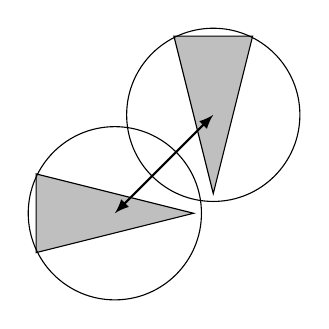
\begin{tikzpicture}[scale=0.5]
  \draw[fill=lightgray] (0,0) -- (0,2) -- (4,1) -- cycle;
  \draw (2,1) circle (2.2);
  \draw[fill=lightgray] (4.5,1.5) -- (3.5,5.5) -- (5.5,5.5) -- cycle;
  \draw (4.5,3.5) circle (2.2);
  \draw[thick,arrows=<->,>=latex] (4.5,3.5) -- (2,1);
\end{tikzpicture}
\hfill
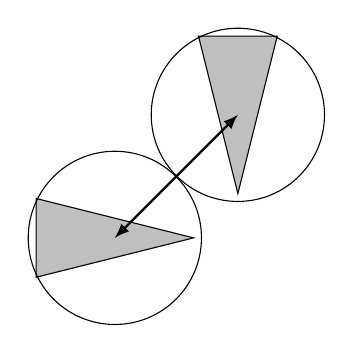
\begin{tikzpicture}[scale=0.5]
  \draw[fill=lightgray] (0,0) -- (0,2) -- (4,1) -- cycle;
  \draw (2,1) circle (2.2);
  \draw[fill=lightgray] (5.125,2.125) -- (4.125,6.125) -- (6.125,6.125) -- cycle;
  \draw (5.125,4.125) circle (2.2);
  \draw[thick,arrows=<->,>=latex] (5.125,4.125) -- (2,1);
\end{tikzpicture}
  
\end{frame}

\bframe{Spatial Partitioning}
\begin{itemize}
\item Partition space into $O(n)$ cells.
\item Each object updates its cell location.
\item Only check for collisions in cells which overlap collision bound
  circle.
\item Reduces $O(n^2)$ to $O(n)$.
\item {\tt Another Big Shoal.exe}
\end{itemize}

\end{frame}

\bframe{Smoothing}
\begin{itemize}
\item Occasionally bots appear to shudder.
\item Different steering takes place every other frame:
  \begin{itemize}
  \item Toward object, away from obstacle, toward object, away from
    obstacle, ...
  \end{itemize}
\item Simple solution:  decouple bot heading from actual velocity.
\item Bot heading is average velocity of last few steps.
\end{itemize}

\end{frame}




\end{document}
